\documentclass[a4paper]{article}

\usepackage[english]{babel}
\usepackage[utf8]{inputenc}
\usepackage{mathtools}
\usepackage{gensymb}
\usepackage{verbatim}
\usepackage{amssymb}
\usepackage{longtable}
\usepackage{amsmath}
\usepackage[thmmarks,amsmath]{ntheorem}
\usepackage{booktabs,siunitx}
\usepackage{graphicx}
\usepackage[colorinlistoftodos]{todonotes}
\usepackage{geometry}
\usepackage{float}
\usepackage{hyperref}
\usepackage{caption}
\usepackage[bottom]{footmisc}
\geometry{
 a4paper,
 total={170mm,257mm},
 left=30mm,
 right=30mm,
 top=20mm,
 }
\author{[[Name]]}
\title{Report - [[Experiment]]}

\begin{document}

% section hkdhgkjh (end)

\maketitle
\abstract 

Almost all electronic devices are based on silicon. The temperature dependence of the resistance of silicon is investigated in this experiment. From this, the band gap energy $E_g$ is calculated from both heating up and cooling down the the sample. The found energies were $E_{h,g} = [[E_g_h]]$ eV for heating up and $E_{c,g} = [[E_g_c]]$ eV for cooling down the silicon sample. These values were found using a regression line through $y=c_1 x + c_2$ with $y = \ln{R}$ and $x = 1/(2 k_B T)$ and a successive analysis of the residual plots to determine the intrinsic regime of the semiconductor. It was found that the two energies $E_{h,g}$ for heating up and $E_{c,g}$ for cooling down differ in a small amount probably due to hysteresis.

\section{Basic properties of semiconductors}
\label{sec:introduction}

Semiconductors are used in industry very versatile. Integrated circuits, such as microprocessors or -controllers, power electronics, transistors, which are the very basic elements to build electronic circuits, that are on their part used to assemble computers. A large amount of physicists around the world are specialized in semiconductor physics.

Semiductors are solids that have electric conductivity values between metals and insulators. The resistance - and thus the conductivity, the charge carrier concentration and the mobility - depend highly on the temperature, as opposed to metals or insulators. The band gaps of semiconductors are much smaller than those of insulators, making it possible for an electron to excite from the valence band to the conduction band. Because of these properties, they form the basis of all modern electronics, such as diodes and transistors. In computers, semiconductors are used in microprocessors, chips or mainboards. In this experiment the resistance of the semiconductor material silicon (Si) and its temperature-dependence is investigated. The most important semiconductors in industry and research are silicon (Si), germanium (Ge). These are found in the carbon group (group 14) of the periodic table of elements. Silicon and germanium are used because they have 4 valence electrons in their outermost shell which gives them the ability to gain or lose electrons equally at the same time \cite{yacobi2003}. Compounds of elements in groups 13 and 15 such as gallium arsenide (GaAs) are also very widespread.

\subsection{Theory}
\label{sec:theory}

The major difference between a semiconductor and a metal is the temperature dependence of its conductivity. The conductivity of metals is usually very high in the regime of $10^5 \frac{1}{\Omega cm}$ decreasing with temperature increasing, but they stay in this regime. Insulators do have a very small conductivity in the regime of $10^{-14} \frac{1}{\Omega cm}$, staying constant, when changing temperature. Semiconductor on the other hand have a conductivity in a much broader range inbetween metals and insulators. The range spans from $10^{-12} \frac{1}{\Omega cm}$ up to $10^3 \frac{1}{\Omega cm}$ and is dependant of the temperature. The conductivity is defined as the reciprocal of the resistivity and usually denoted by a sigma $\sigma = \frac{1}{R}$.

\subsubsection{The valence and conduction bands}

To describe the electronic properties of a material, the electronic band structure is very useful. It describes the range of energy an electron within a solid can or cannot have. The energy it cannot have is called the band gap. The band structure is derived using the Schroedinger equation of an electron in a crystal. Since the exact form of the potential in the solid is not known the potential is approximated using the approximation of the quasi free electron. In figure \ref{fig:scheme} a scheme of the band structure can be seen for metals, insulators and semiconductors. The Fermi-energy $E_F$ is the energy which separates the occuppied from the unoccupied states when the quantum-mechanical system is in ground state. In a metal the Fermi-energy lies inside one or more allowed bands. The names of the bands near the Fermi-energy are conduction and valence band - these are the most important bands and band gap for electronics.

\begin{figure}
\captionsetup{singlelinecheck=off}
\centering
\includegraphics[width=0.6\textwidth]{img/scheme.jpg}
\caption[blubb]{Scheme of the energies of metals (left), semiconductors (center) and insulators (right). For semiconductors and insulators the Fermi-energy $E_F$ lies between the valence and the conduction bands terminated by the energies $E_V$ for the upper limit of the valence band and $E_L$ for the lower limit of the conduction band. Metals do have a partially occupied band. Source: \cite{esslin2018}}
\label{fig:scheme}
\end{figure}

\subsubsection{The band gap}

A band gap is a special range between the conduction and the valence band of a semiconductor where no electron can exist. The band gap energy $E_g$ is therefore the energy difference between the bottom of the conduction band and the top of the valence band and thus the energy needed for a valence electron to become a conduction electron, which participates to the current trough the material. The band gap energy is therfore $E_L - E_V$ according to figure \ref{fig:scheme} (Note that later in the report the upper limit of the valence band is called $E_V$ and the lower limit of the conduction band is called $E_C$).

\subsubsection{The doped semiconductor}

Doping a semiconductor means intentially introduce impurities to the semiconductor material. The purpose of this is manipulating the electric properties. Doping allows energy states within the band gap of the pure semiconductor. There are two types of doping; when the dopant atom is a an electron donor, there is a region in the semiconductor that can form an n-type region. That is a region where there are more electrons than holes, raising the Fermi-energy closer to the conduction band. The charge carrier density of the electrons $n$ is then grather than the charge carrier density of holes $p$. When the dopant atom is an electron acceptor, a region of less electrons can be formed (more holes than electrons), called a p-type region. The Fermi-energy lowers closer to the valence band in this case and $p > n$. A semiconductor can be doped with donors and acceptors in the same way, such that the charge carrier density of electron and holes stay the same $n=p$, thus the semiconductor is still intrinsic, but not pure. Since the donor and acceptor electron sit very close to the band gap edges, it is much easier to thermally excite such an electron to the conduction band. Even if the temperature is too small to excite an electron from the valence to the conduction band, it might be enough for the donor electron to be excited. This is extrinsic conduction and the semiconductor is called to be extrinsic.

\subsubsection{The intrinsic regime}

When the temperature is raising, the first electrons, which get excited, are the donor electrons. This is called the extrinsic conduction. After all donor electrons are excited and the temperature is still increasing, the electrons from the valence band start go get excited to the conduction band. When this dominates, the conduction is called intrinsic. A doped semiconductor has a regime of temperature - called the intrinsic regime - where all donor electrons are excited and the dominant excitation is from valence electrons. In that regime, the electron and hole densities are equal $n=p$. Using the Fermi-Dirac distribution for the probability that the states are occipied by charge carriers and $E_C - E_F \gg k_B T$ and $E_F - E_V \gg k_B T$, we get

\begin{subequations}
\begin{align}
    n &= N_C(T) \exp{\left(-\frac{E_C - E_F}{k_B T} \right)} \label{eq:n} \\
    p &= N_V(T) \exp{\left(\frac{E_V - E_F}{k_B T} \right)} \label{eq:p}
\end{align}
\end{subequations}

with $N_{C,V} \propto T^{3/2}$ the effective density of states. Using $n p = n_i^2$ (because of $n=p$, $i$ stands for intrinsic) and the definition $E_g = E_C - E_V$, we find that 

\begin{equation}
n_i \propto T^{3/2} \exp{\left( -\frac{E_g}{2 k_B T} \right)} \label{eq:ni}
\end{equation}

We know that the conductivity holds the relation $\sigma = n e \mu$, where $n$ is the charge carrier density, $e$ is the elementary electron charge and $\mu$ the mobility. Using (\cite{seitz1952})

\begin{subequations}
\begin{align}
\frac{1}{\mu} &= \alpha_l T^{3/2} + \alpha_i T^{-3/2} + \alpha_d T^{-1} \label{eq:seitz} \\
\implies \mu &\propto T^{-3/2} \label{eq:mu} \\
\end{align}
\end{subequations}

only considering acoustic phonons \cite{esslin2018}. Using this, one can find the temperature dependence of the conductivity using the band gap energy $E_g$:

\begin{equation}
\sigma = \frac{1}{R_S} \propto \exp{\left( - \frac{E_{g}}{2 k_B T} \right)} \label{eq:conductivity}
\end{equation}

where $R_S$ is the resistivity of the sample (the semiconductor). These are now relations only between measureable ($R_S$, $T$) or known ($k_B$) quantities.

\subsection{Four-probe-measurement}
\label{sec:fpm}

To measure the voltage and calculate the resistance, the method called four-probe-measurement is used. In four-probe-measurement, the current-carrying and voltage-sensing electrodes were separated. This eleminates the wire- and contact-resistance from the measurement. Specially when measuring low resistance values, this technique is prefered over the more usual two-probe-measurement method, because the resistance of the circuit is not added to the resistance of the sample under test. In figure \ref{fig:fourprobe} a circuit for the four-probe-measurement can be seen. The resistances $R_1$, $R_2$, $R_3$ and $R_4$ represent resistances in the wires and the contacts to the sample with the resistance of interest $R_S$. $R_V$ is the internal resistance of the voltmeter $V$. The voltmeter should have a high - ideally infinite - resistance itself. Therfore the resistance of the contact to the sample becomes less important. The voltage sensing leads should be connected as close to the resistor under test as possible to avoid including the resistance of the test leads in the measurement \cite{llmh}. The current through the voltmeter $i_V$ should be negligible. The sample is under constant current supply $i_0$. Therefore there is nearly no current flowing through the sensing wires ($i_V \ll i_0$) and thus it arises nearly no voltage drop ($i_V \left( R_2 + R_3 \right) \ll i_0 R_S$). When $V_4$ is the measured voltage over the voltmeter, the resistance $R_S$ can then be calulated by

\begin{equation}
R_S \approx \frac{V_4}{i_0}.
\end{equation}

The approximation holds when the above assumptions hold ($i_V \ll i_0$ and $i_V \left( R_2 + R_3 \right) \ll i_0 R_S$).

\begin{figure}[H]
\captionsetup{singlelinecheck=off}
\centering
\includegraphics[width=0.6\textwidth]{img/fourprobe.jpg}
\caption[blubb]{A schematic of the four-probe-measurement method. Source: \cite{inst2014}}
\label{fig:fourprobe}
\end{figure}

\section{Setup}

The experimental setup is despicted in figure \ref{fig:setup}. The pump to evacuate the oven (vacuum tube) is not visible in the picture, but there is a pipe connected to the oven. The pump was under the table seen in the picture. The device labeled with ($4$) in the picture is the display for the temperature inside the tube. It is connected by the green wire to a thermocouple device. The gray cable comming from the oven, splits up into 4 separate wires. These are for the four-probe-measurement (see section \ref{sec:fpm}). The multimeter labeled with ($8$) is used to read the voltage of the power supply and set the operating point (see section \ref{sec:operating_point}). Starting with room temperature, the sample was heaten up until $900 K$ and then cooled down until around $400 K$. One measurement consisted of taking the voltage $V_4$ and the current $I$ over four-probe-measurement for temperature steps of $5 K$.

\begin{figure}[H]
\captionsetup{singlelinecheck=off}
\centering
\includegraphics[width=1.0\textwidth]{img/setup.jpg}
\caption[blubb]{Image of the experimental setup. The device labeled with ($1$) is to configure the pump (not in the picture) and to display the pressure, ($2$) is the device to set the current through the vacuum tube ($3$) and thus to raise and lower the temperature inside, ($4$) is the display of the thermocouple displaying the temperature inside the tube, ($5$) is the power suppy, ($6$) and ($7$) are the devices to read off the current $I$ and the voltage $V_4$, ($8$) is a multimeter adjusted to measure control voltage over the power supply. The pump was turned on by a switch at the power socket ($9$). Source: Authors' own.}
\label{fig:setup}
\end{figure}

\section{Measurement Method}

\subsection{Evacuating the oven}

In a first step the oven with the semiconductor material inside was evacuated to a pressure, such that the sample will not oxidize. Else the contact with the wires would be bad and therefore result in a systematic error in the measurement data. This took around $20$ minutes.

\subsection{Operating point}
\label{sec:operating_point}

To find the optimal current regime for the experiment, the four-probe resistance and temperature of the sample were measured as a function of the current applied to the sample (see figure \ref{fig:operating_point}). In the graph there is a region hightlighted as "safe zone", this is where the temperature and the resistance are still constant in current. This zone determines the optimal current regime. The operating point was chosen to be $I_{Op} = [[I_Op]] \, mA$, which corresponds to a voltage $V_{2,Op} = [[V_2_Op]] \, V$ (see figure \ref{fig:operating_point}). For the measured data, plase refer to table \ref{tab:operating_point} in the appendix.

\begin{figure}[H]
\captionsetup{singlelinecheck=off}
\centering
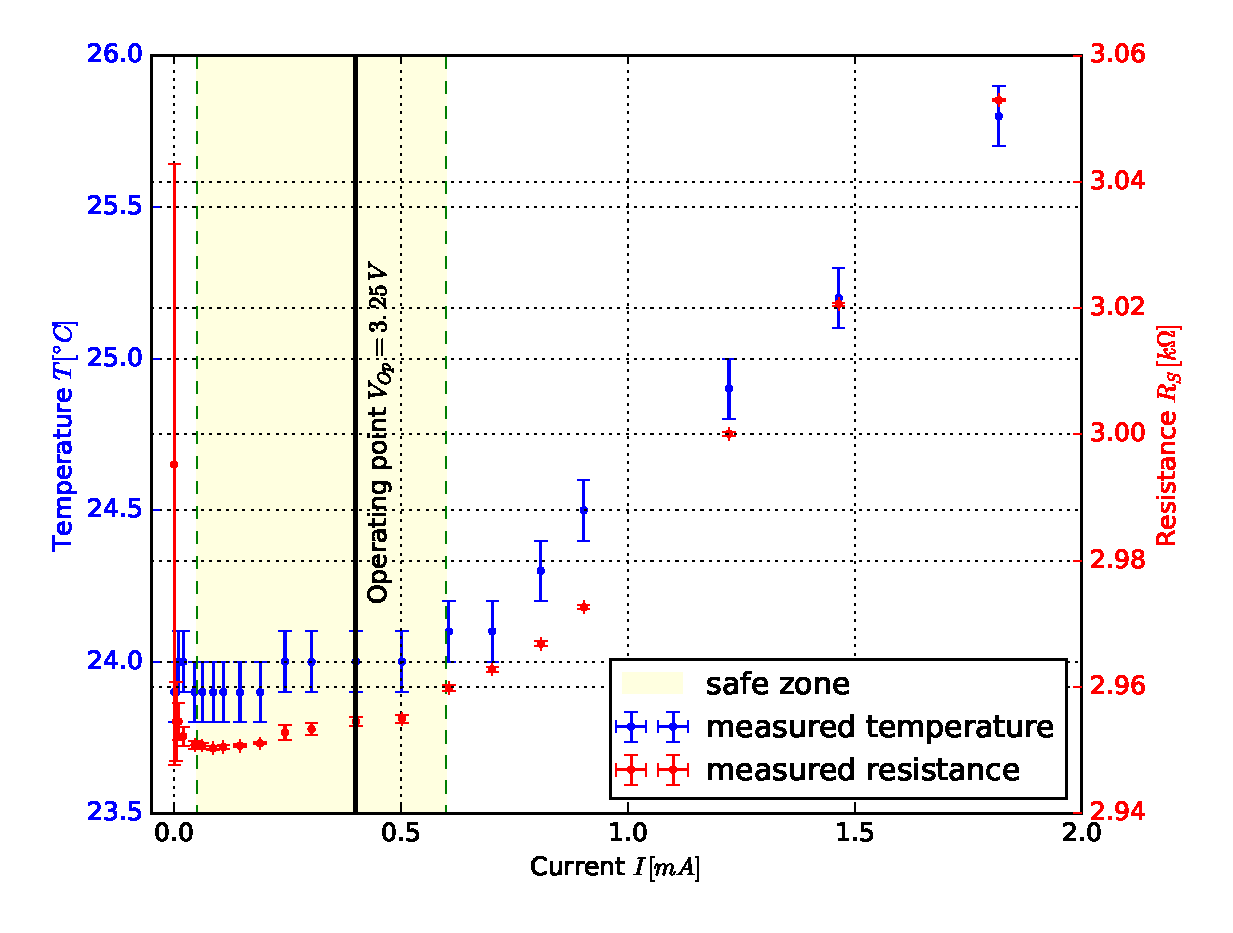
\includegraphics[width=1.0\textwidth]{plots/operating_point.eps}
\caption[blubb]{Plot of temperature and resistance of the sample against current applied to the sample to determine the opernating point of the experiment. The yellow area labeled with "safe zone" defines the interval in current (voltage) where the optimal current regime is, thus the operating point can be chosen. Source: Authors' own.}
\label{fig:operating_point}
\end{figure}

\subsection{Four-probe-measurement}

To measure the resistance of the sample as a function of the temperature, the vacuum tube was heaten up from room temperature ($\approx 300 K$) to $\approx 900 K$, afterwards is was cooled down back to room temperature. During this procedure, the resistance was measured in steps of $5 K$. To measure the resistance, the method of the four-probe-measurement was used.
\newline
For this, the current $I$ and the voltage $V_4$ were measured. The resistance $R_S$ can then simply be calculated using Ohms law

\begin{equation}
R_S = \frac{V_4}{I}.
\end{equation}

\subsection{Calculating the band gap energy $E_g$}

Since the conductivity $\sigma$ is the reziprocal of the resistance $R_S$ and the conductivity meets equation \eqref{eq:conductivity}, the band gap energy $E_g$ can be calculated as the leading coefficient of a linear interpolation of the measured data

\begin{equation}
y = c_1 x + c_2
\end{equation}

with $y = \ln{R_S}$ and $x = \frac{1}{2 k_B T}$. The band gap energy would then be the coefficient $c_1$. For this to hold, the intrinsic regime of the semiconductor must be determined first, because equation \eqref{eq:conductivity} only holds in that regime.

\subsection{Determining the instrinsic regime}
\label{sec:intrinsicRegime}

Since the deduction of the band gap energy involves a linear regression line of the measured data, one possibility to localize the intrinsic regime is to inspect the residuals of that line. In a first step all measured data were used for the regression line, unsuprisingly the residual plot displayed a linear-shaped pattern, suggesting that the linear regression is not justified (see figure \ref{fig:residuals} left). In a second step, the two plots (\ref{fig:energy_gap}) were inspected by eye to see where the data starts to be non-linear. The two bounds for the instrinsic regime $B_{\downarrow}$ and $B_{\uparrow}$ were set accordingly. The resudual plot still showed a U-shape (see figure \ref{fig:residuals} center), but it was visible in the plot, where the U began to be shaped, indicating that there was data with a random pattern. So after taking the residual plot into account and analyzing their patterns, the two bounds for the intrinsic regime could be found appropriately in a final third step (see figure \ref{fig:residuals} right). The mean and the sum of the residual are also very close to zero, indicating that the two bounds were chosen correctly. They are as follows, for each step (where $e_1$, $e_2$ and $e_3$ are the residuals of step $1$, $2$ and $3$, $e_h$ and $e_c$ are the residuals for heating and cooling respectively):

\begin{itemize}
	\item Step 1
	\begin{itemize}
		\item Mean: $\overline{e_{1,h}} = [[res:mean:h:step1]]$
		\item Mean: $\overline{e_{1,c}} = [[res:mean:c:step1]]$
		\item Sum: $\sum {e_{1,h,i}} = [[res:sum:h:step1]]$
		\item Sum: $\sum {e_{1,c,i}} = [[res:sum:c:step1]]$
	\end{itemize}
	\item Step 2
	\begin{itemize}
		\item Mean: $\overline{e_{2,h}} = [[res:mean:h:step2]]$
		\item Mean: $\overline{e_{2,c}} = [[res:mean:c:step2]]$
		\item Sum: $\sum {e_{2,h,i}} = [[res:sum:h:step2]]$
		\item Sum: $\sum {e_{2,c,i}} = [[res:sum:c:step2]]$
	\end{itemize}
	\item Step 3
	\begin{itemize}
		\item Mean: $\overline{e_{3,h}} = [[res:mean:h:step3]]$
		\item Mean: $\overline{e_{3,c}} = [[res:mean:c:step3]]$
		\item Sum: $\sum {e_{3,h,i}} = [[res:sum:h:step3]]$
		\item Sum: $\sum {e_{3,c,i}} = [[res:sum:c:step3]]$
	\end{itemize}
\end{itemize}

\begin{figure}[H]
	\captionsetup{singlelinecheck=off}
	\centering
	\begin{minipage}[t]{0.3\textwidth}
		\begin{center}
		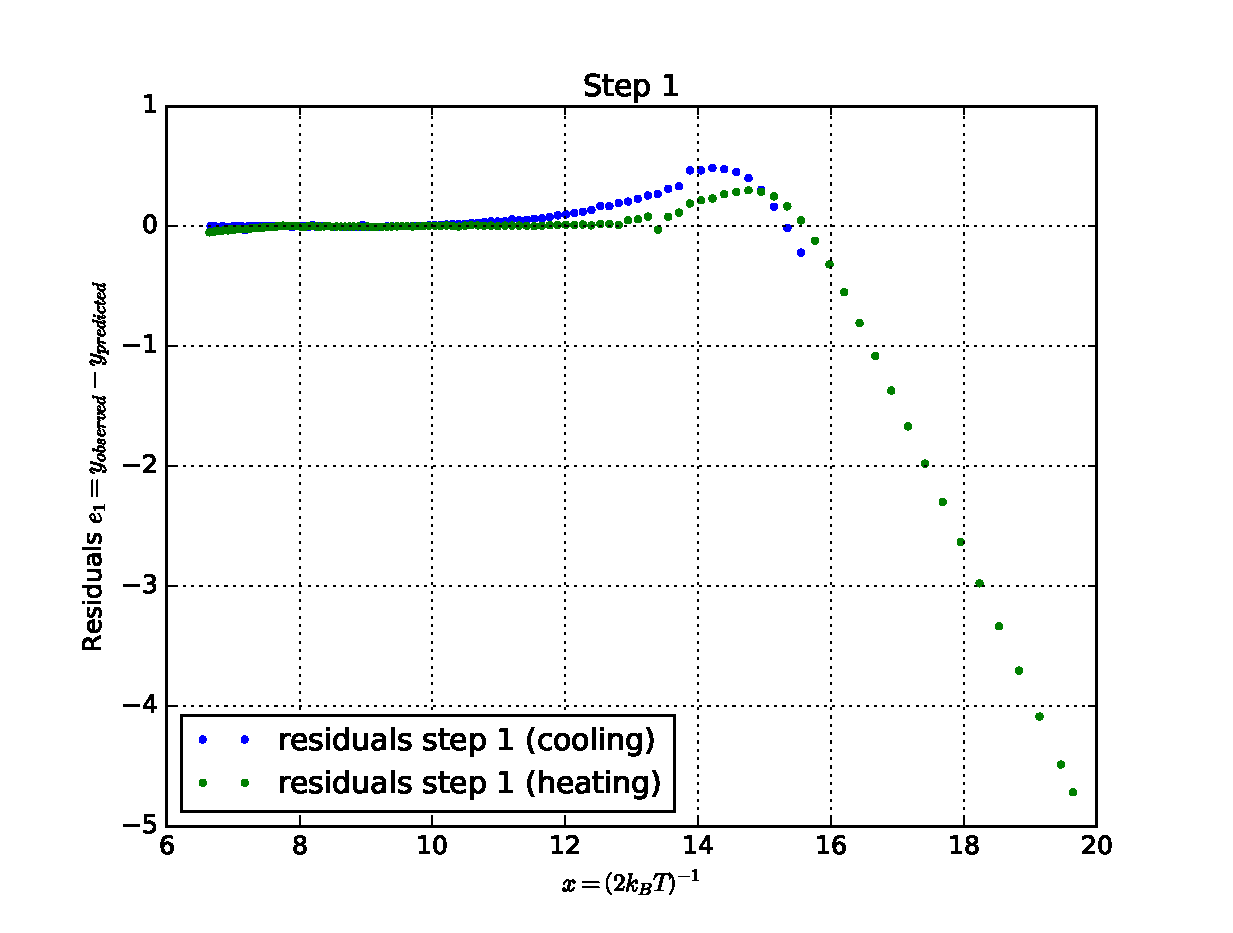
\includegraphics[width=1.0\textwidth]{plots/residuals_step1.eps}
		\end{center}
	\end{minipage}
	\begin{minipage}[t]{0.3\textwidth}
		\begin{center}
		\includegraphics[width=1.0\textwidth]{plots/residuals_step2.eps}
		\end{center}
	\end{minipage}
	\begin{minipage}[t]{0.3\textwidth}
		\begin{center}
		\includegraphics[width=1.0\textwidth]{plots/residuals_step3.eps}
		\end{center}
	\end{minipage}
	\caption[blubb]{The resudual plots for the 3 steps in finding the instrinsic regime. Both the sum and the mean of the residuals should be zero. Source: Authors' own.}
	\label{fig:residuals}
\end{figure}

\section{Measurements and Discussion}

\subsection{Evacuating the oven}

The oven was evacuated to a pressure of $p = 3.5 \times 10^{-2}$ mbar. However this pressure changed a bit during the experiment, because the pump was not turned off (the pressure would rapidly increase, if that would have been done). So the pressure slowly changed to a value of $p = 1.2\times 10^{-2}$ mbar at the end of the experiment. The impact of this was neglected.

\subsection{Operating point}

As seen in the analysis of the operating point (see section \ref{sec:operating_point}), the current of operation was chosen to be $I_{Op} = [[I_Op]]$ mA. This corresponds to a voltage of $V_{2,Op} = [[V_2_Op]]$ V.

\subsection{Temperature dependence of the resistance}

In figure \ref{fig:temperature_resistance}, the temperature $T$ is plotted against the resistance $R_S$ of the sample. It can be seen that the resistance increases when temperature increases, up until a point at  $\approx 370 K$ where it decreases very fast and finally approaches zero for temperatures higher than $600 K$.

\begin{figure}[H]
\captionsetup{singlelinecheck=off}
\centering
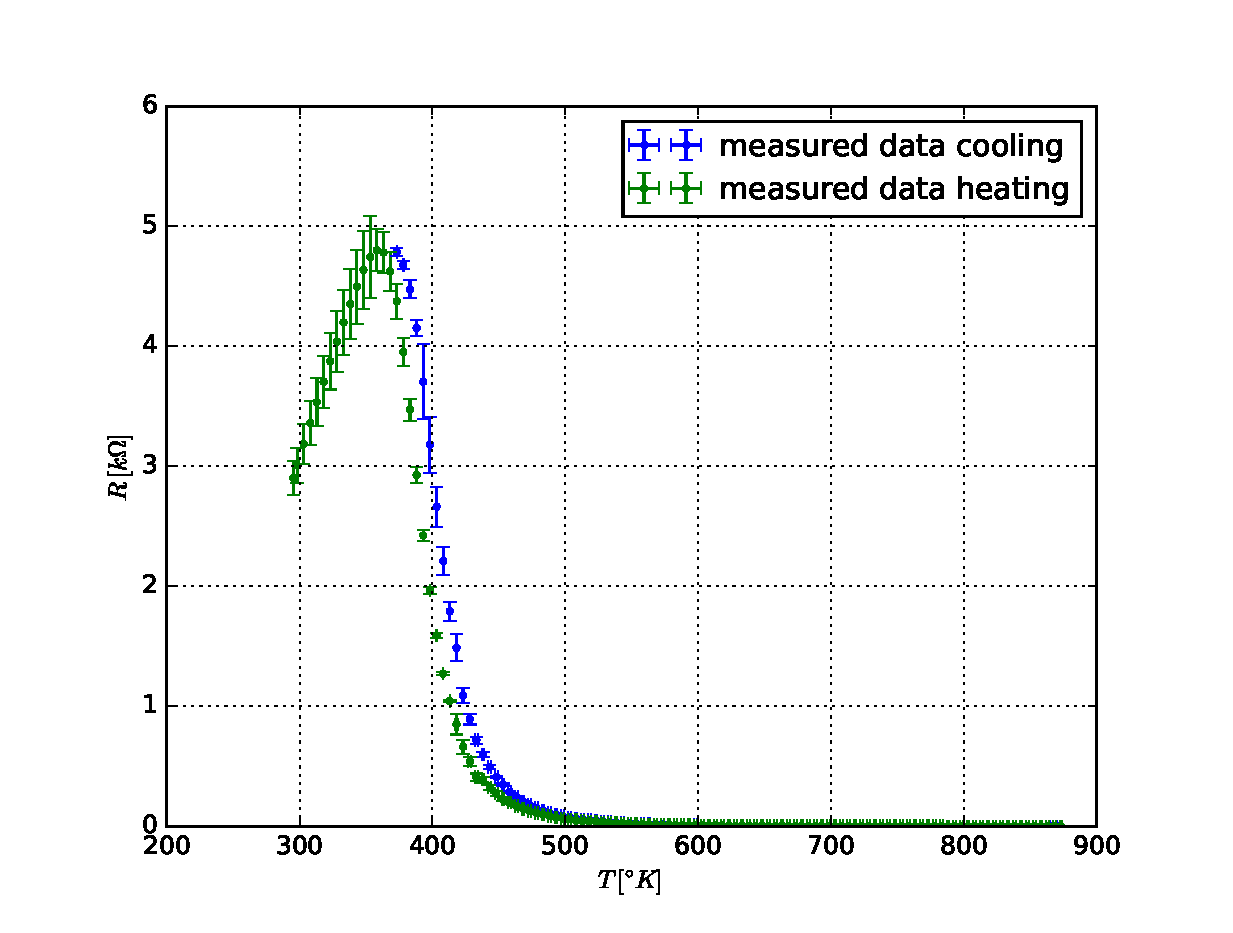
\includegraphics[width=1.0\textwidth]{plots/temperature_resistance.eps}
\caption[blubb]{Resistance $R_S$ as a function of temperature $T$ of the sample. The marked bounds $T_{\uparrow}$ and $T_{\downarrow}$ delimit the intrinsic regime for cooling and heating respectively. Source: Authors' own.}
\label{fig:temperature_resistance}
\end{figure}

\subsection{Energy gap}

To find the band gap energy $E_g$ of silicon, it was necessary to determine the intrinsic regime of the semiconductor (see section \ref{sec:intrinsicRegime}). The intrinsic regime is between the two bounds $B_{\downarrow}$ and $B_{\uparrow}$; these are as follows

\begin{subequations}
\begin{align}
B_{\downarrow} &= [[B_lower_h]] \, eV &\implies T_{\uparrow} = [[T_upper_h]] \, K\\
B_{\uparrow} &= [[B_upper_h]] \, eV &\implies T_{\downarrow} = [[T_lower_h]] \, K
\end{align}
\end{subequations}

for the heating process (see figure \ref{fig:energy_gap} green) and 

\begin{subequations}
\begin{align}
B_{\downarrow} &= [[B_lower_c]] \, eV &\implies T_{\uparrow} = [[T_upper_c]] \, K \\
B_{\uparrow} &= [[B_upper_c]] \, eV &\implies T_{\downarrow} = [[T_lower_c]] \, K
\end{align}
\end{subequations}

for the cooling process (see figure \ref{fig:energy_gap} blue). Once that regime was identified, the band gap energy could be calculated using a linear regression line through the measured data and its coefficients $c_1$ and $c_2$ (see figure \ref{fig:energy_gap} green for the calculation with data from heating up and figure \ref{fig:energy_gap} blue for the calculation with data from cooling down the sample). The linear regression lines are as follows:

\begin{subequations}
\begin{align}
p_{h}(x) &= [[linear_fit_h]] \\
p_{c}(x) &= [[linear_fit_c]]
\end{align}
\end{subequations}

where $p_h(x)$ and $p_c(x)$ are the linear regression lines for heating and cooling respectively. Thus the band gap energies can be read off. The band gap energies for heating and cooling are (see figure \ref{fig:energy_gap}):

\begin{subequations}
\begin{align}
E_{g,heating} &= [[E_g_h]] \, eV \label{eq:egh} \\
E_{g,cooling} &= [[E_g_c]] \, eV \label{eq:egc}
\end{align}
\end{subequations}

\begin{comment}
\begin{figure}[H]
	\begin{minipage}[t]{0.5\textwidth}
		\begin{center}
		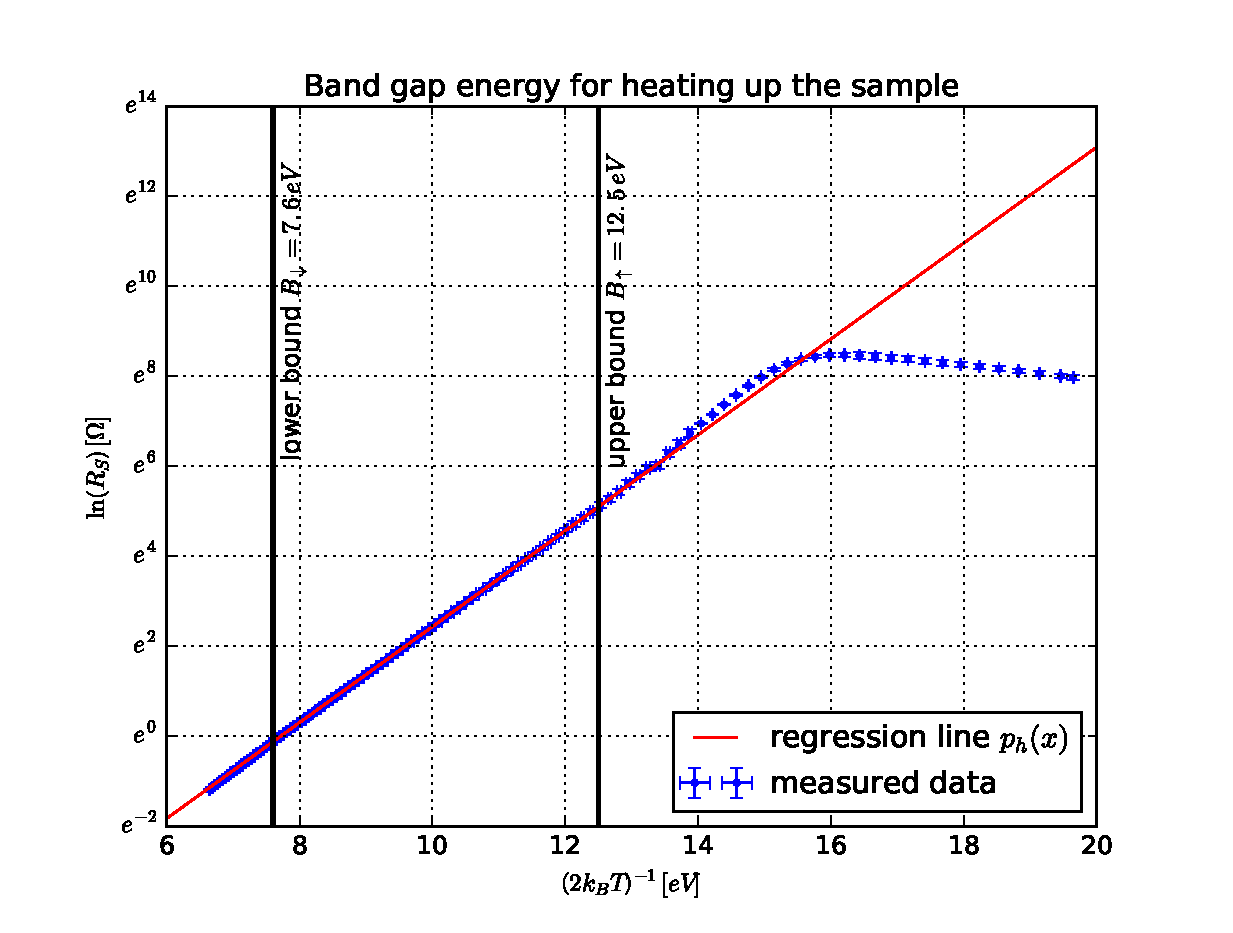
\includegraphics[width=1.0\textwidth]{plots/energy_gap_heating.eps}
		\end{center}
	\end{minipage}
	\begin{minipage}[t]{0.5\textwidth}
		\begin{center}
		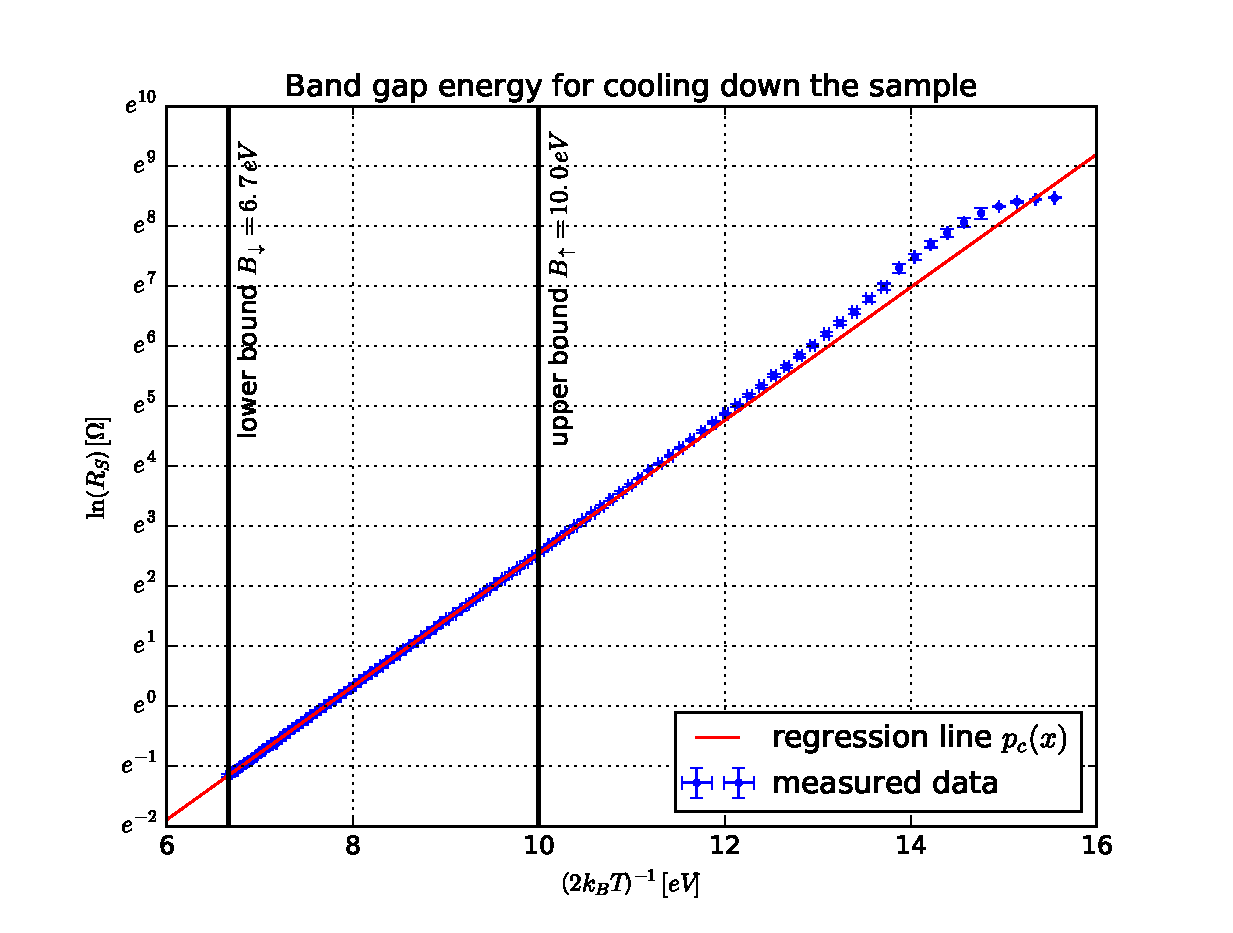
\includegraphics[width=1.0\textwidth]{plots/energy_gap_cooling.eps}
		\end{center}
	\end{minipage}
	\caption{Plot of the natural logarithm of the sample resistance $\ln{\left( R_S \right)}$ against the inverse temperature $\left(2 k_B T \right)^{-1}$ scaled by $2$ times the Boltzmann constant $2 k_B$ to identify the slope of the regression line (red). The upper and lower bounds used for the regression line for heating (left) are $B_{\downarrow} = [[B_lower_h]] \, eV$ and $B_{\uparrow} = [[B_upper_h]] \, eV$ and for cooling (right) are $B_{\downarrow} = [[B_lower_c]] \, eV$ and $B_{\uparrow} = [[B_upper_c]] \, eV$. The regression lines: $p_h(x) = [[linear_fit_h]]$ and $p_c(x) = [[linear_fit_c]]$. Source: Authors' own.}
	\label{fig:energy_gap}
\end{figure}
\end{comment}

\begin{figure}[H]
\captionsetup{singlelinecheck=off}
\centering
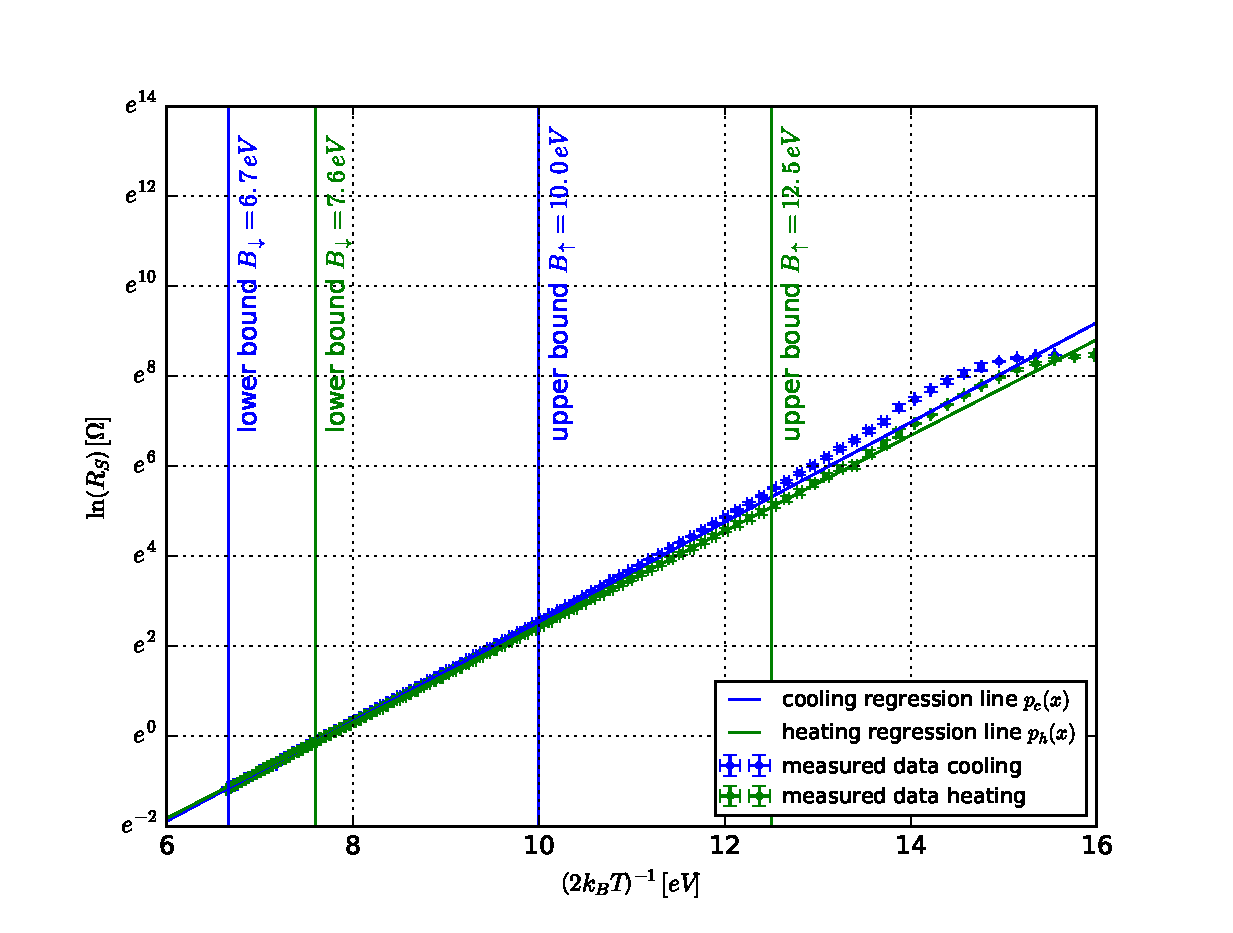
\includegraphics[width=1.0\textwidth]{plots/energy_gap.eps}
\caption[blubb]{Plot of the natural logarithm of the sample resistance $\ln{\left( R_S \right)}$ against the inverse temperature $\left(2 k_B T \right)^{-1}$ scaled by $2$ times the Boltzmann constant $2 k_B$ to identify the slope of the regression lines. The upper and lower bounds used for the regression line for heating (green) are $B_{\downarrow} = [[B_lower_h]] \, eV$ and $B_{\uparrow} = [[B_upper_h]] \, eV$ and for cooling (blue) are $B_{\downarrow} = [[B_lower_c]] \, eV$ and $B_{\uparrow} = [[B_upper_c]] \, eV$. In the figure, the difference in the slope of the two regression lines can be seen. The regression lines are: $p_h(x) = [[linear_fit_h]]$ and $p_c(x) = [[linear_fit_c]]$. Source: Authors' own.}
\label{fig:energy_gap}
\end{figure}

The two energies $E_{g,heating}$ and $E_{g,cooling}$ differ. Thus the measured band gap energy between the conduction and the valence band differs when heating up or cooling down the silicon sample in the regime of intrinsic conduction. The energy to excite an electron from the valence band to the conduction band is lower when the silicon sample is heated up as when it is cooled down. This suggests that there is hysteresis happening here, because the value of the slope of the regression line depends on the direction of change of the temperature.

\begin{comment}
\begin{figure}[H]
\captionsetup{singlelinecheck=off}
\centering
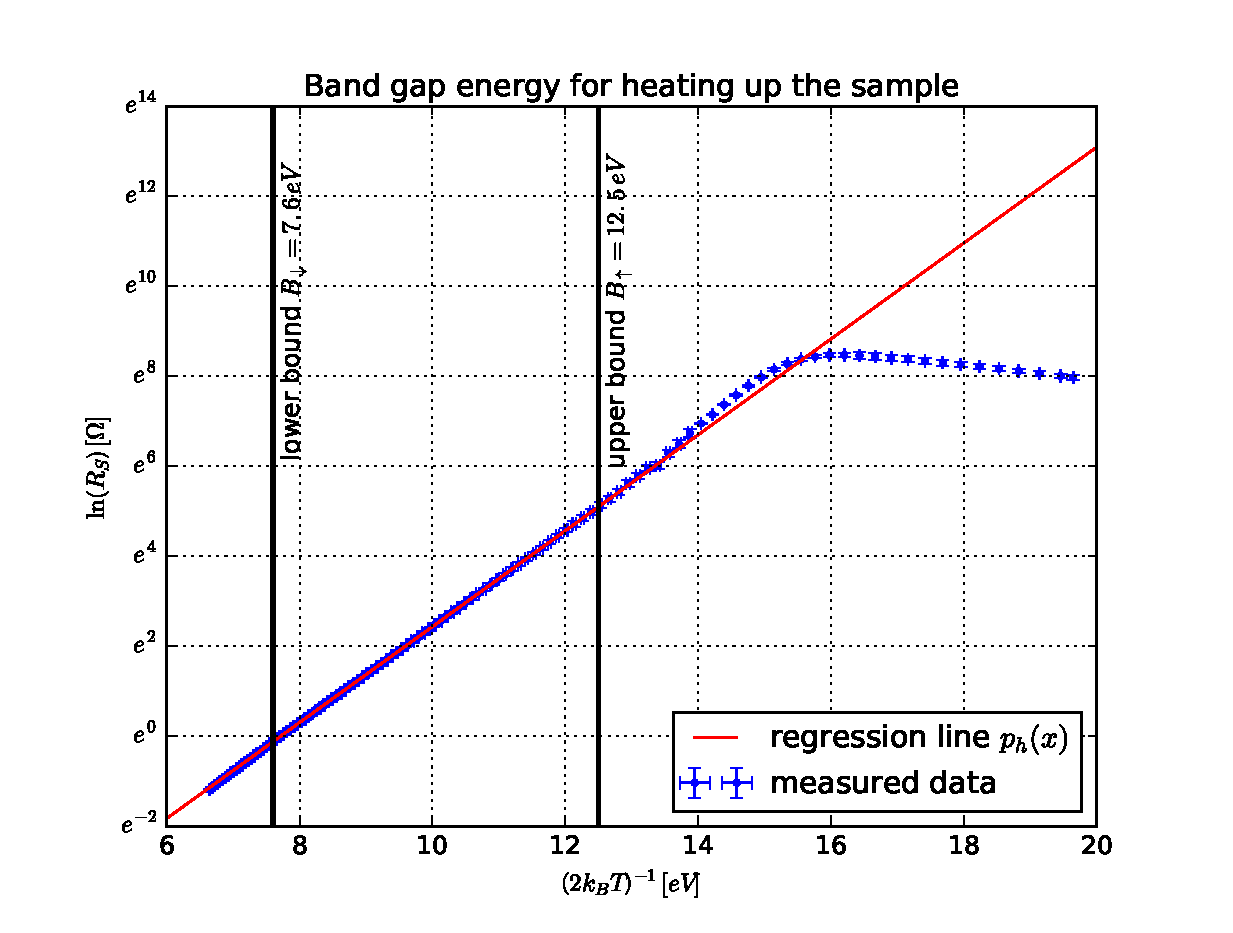
\includegraphics[width=1.0\textwidth]{plots/energy_gap_heating.eps}
\caption[blubb]{Plot of the natural logarithm of the sample resistance $\ln{\left( R_S \right)}$ against the inverse temperature $\left(2 k_B T \right)^{-1}$ scaled by $2$ times the Boltzmann constant $2 k_B$ to identify the slope of the regression line (red). The upper and lower bounds used for the regression line are $B_{\downarrow} = [[B_lower_h]] \, eV$ and $B_{\uparrow} = [[B_upper_h]] \, eV$. The regression line: $p_h(x) = [[linear_fit_h]]$ Source: Authors' own.}
\label{fig:energy_gap_heating}
\end{figure}

\begin{figure}[H]
\captionsetup{singlelinecheck=off}
\centering
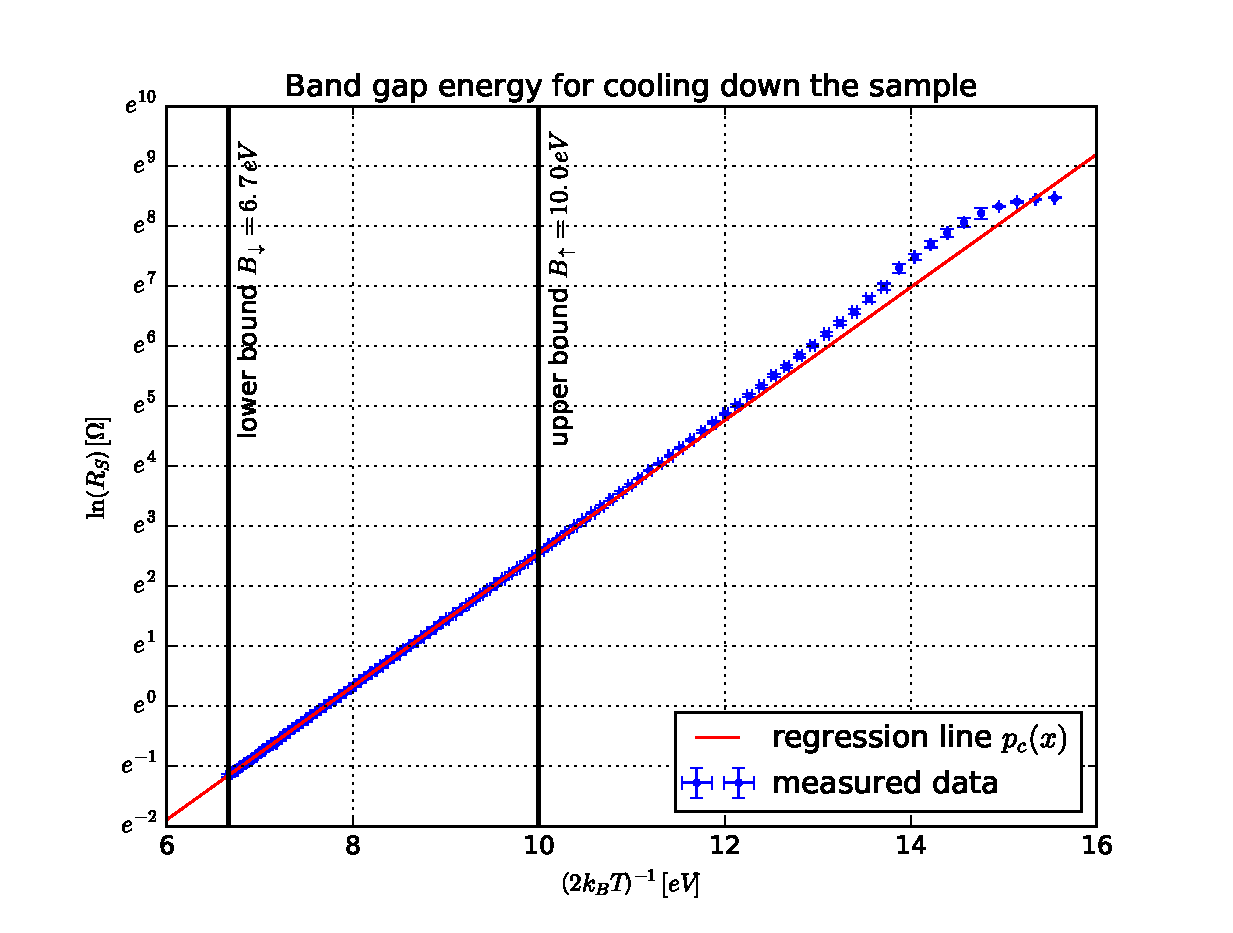
\includegraphics[width=1.0\textwidth]{plots/energy_gap_cooling.eps}
\caption[blubb]{Plot of the natural logarithm of the sample resistance $\ln{\left( R_S \right)}$ against the inverse temperature $\left(2 k_B T \right)^{-1}$ scaled by two times the Boltzmann constant $2 k_B$ to identify the slope of the regression line (red). The upper and lower bounds used for the regression line are $B_{\downarrow} = [[B_lower_c]] \, eV$ and $B_{\uparrow} = [[B_upper_c]] \, eV$. The regression line: $p_c(x) = [[linear_fit_c]]$ Source: Authors' own.}
\label{fig:energy_gap_cooling}
\end{figure}
\end{comment}

\subsection{Mobility and carrier density}

According to the theory (see section \ref{sec:theory}), the carrier density and the mobility in the intrinsic regime have the forms (equations \eqref{eq:ni} and \eqref{eq:mu})

\begin{subequations}
\begin{align}
n_i &\propto T^{3/2} \exp{\left( -\frac{E_g}{2 k_B T} \right)} \\
\mu &\propto T^{-3/2}
\end{align}
\end{subequations}

Figure \ref{fig:theory} displays the calculated forms of these quantities. On the left side there is the calculated mobility $\mu$ plotted against the temperature $T$ and on the right side there is the carrier concentration $n_i$ plotted against the inverse of the temperature $1/T$. It can be seen that the plots  honour the theory.

\begin{figure}[H]
	\begin{minipage}[t]{0.5\textwidth}
		\begin{center}
		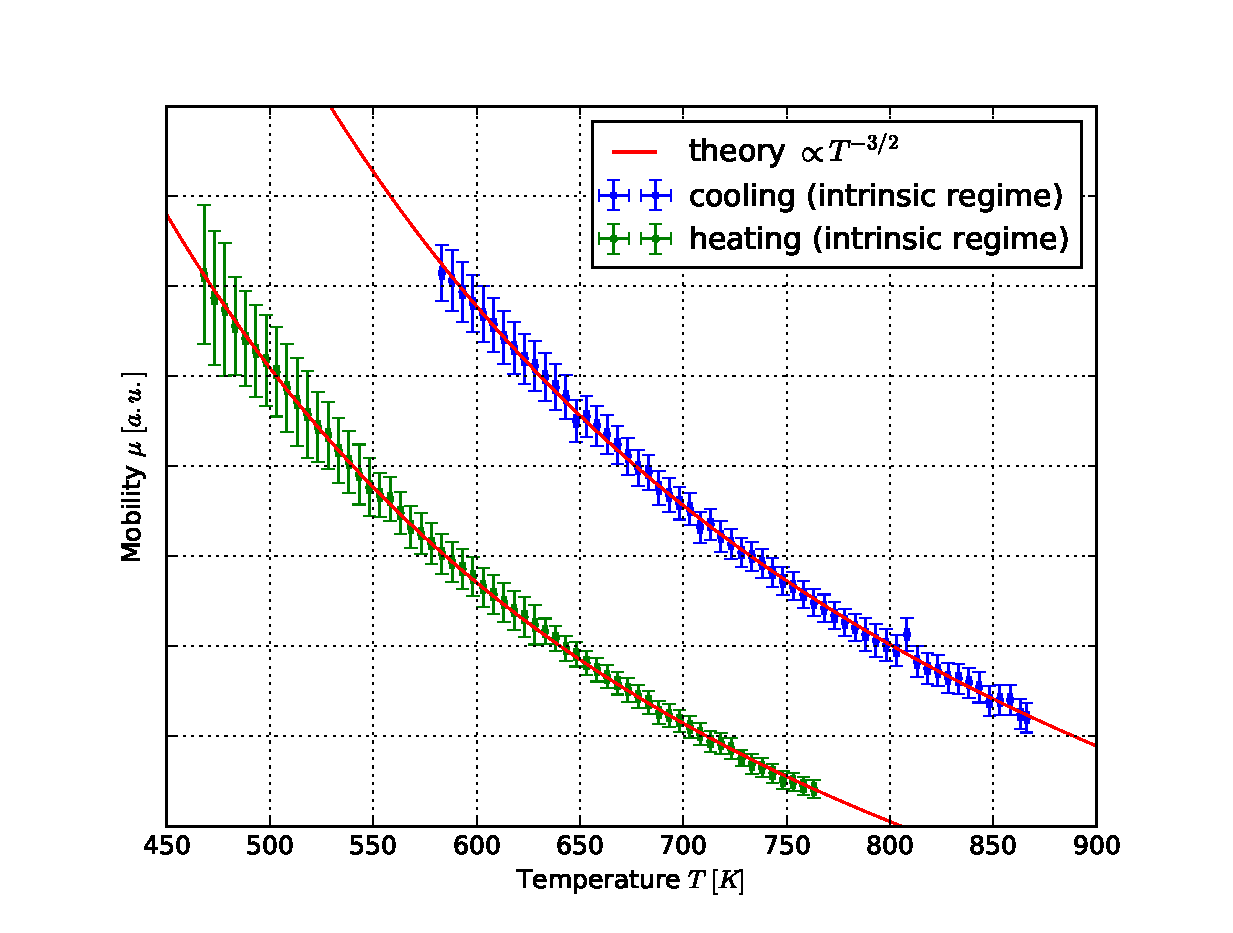
\includegraphics[width=1.0\textwidth]{plots/mobility_vs_temp.eps}
		\end{center}
	\end{minipage}
	\begin{minipage}[t]{0.5\textwidth}
		\begin{center}
		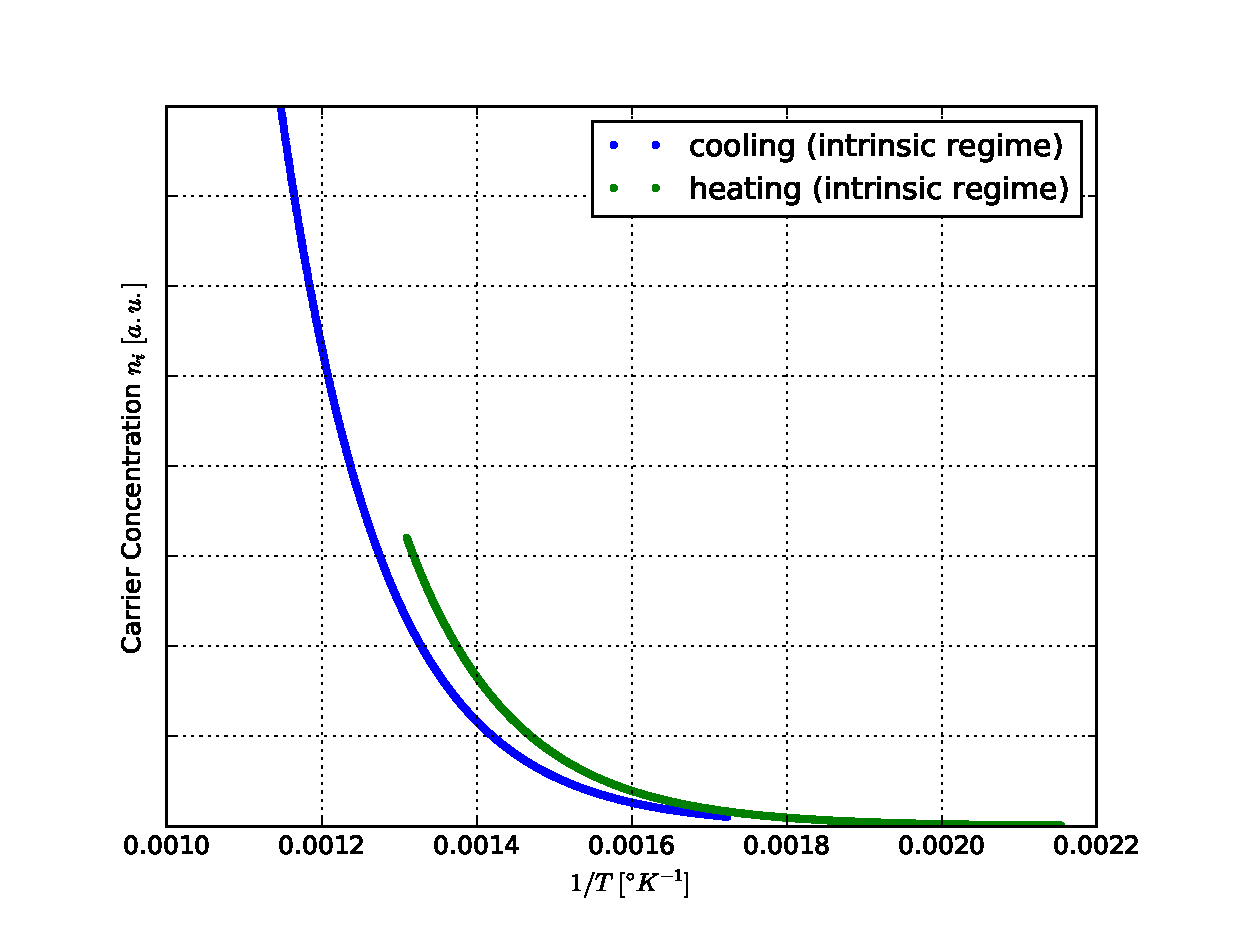
\includegraphics[width=1.0\textwidth]{plots/n_vs_temp_inverse.eps}
		\end{center}
	\end{minipage}
	\caption{Plot of mobility $\mu$ against the temperature $T$ (left) and carrier concentration $n_i$ against the inverse temperature $1/T$ (right), both only plotted in the instrinsic regime. Source: Authors' own.}
	\label{fig:theory}
\end{figure}

\subsection{Errors}

\subsubsection{Operating point}

For finding the operating point (see table \ref{tab:operating_point}), the error for the temperature was chosen to be $\Delta T = 0.1 K$, because the scale of the measuring device was up to one significant figure after the comma. In the measurements of $I$, the scale at the measuring device had to be changed, therefore the error changed from $\Delta I = 0.01 \, \mu A$ to $\Delta I = 0.1 \, \mu A$. The same happend during measurement of the voltage $V$; the error spans from $\Delta V = 1 \, \mu V$ to $\Delta V = 100 \, \mu V$.

\subsubsection{Energy gap}

The measurements to determine the band gap energy $E_g$ were around $220$ single measurements. The scale of the measured quantities changed various times. The error for the temperature was chosen to be $\Delta T = 0.1 K$ for measurements under $140^{\circ}C$ and $\Delta T = 1 K$ for measurements over $140^{\circ}C$. The error values for the voltage $V_4$ and the current $I$ were recalculated multiple times. The procedure was as follows: the voltage and current measurements were taken to be $V_{4,a}$ and $I_a$ and after $2 \cdot \Delta T$ another measurement was taken to be $V_{4,b}$ and $I_b$. The total error for these two quantities was then calculated as

\begin{subequations}
\begin{align}
\Delta V_4 &= \frac{1}{2} | V_{4,b} - V_{4,a} | \\
\Delta I &= \frac{1}{2} | I_b - I_a |
\end{align}
\end{subequations}

$\Delta V_4$ and $\Delta I$ were then rounded up, with respect to the order of magnitude. The exact values can be read from the tables \ref{tab:heating} and \ref{tab:cooling}. This was done every time the scale of a measuring device needed to be changed or all $10-20$ measurements passed (whatever happend first).

\subsection{Systematic error sources}
\label{sec:systematic_errors}

In this experiment there are some sources of systematic errors that were neglected.

\begin{itemize}
\item When changing the temperature of the sample, it was observed that heating was much faster than cooling down. Therefore when heating up the sample, there was a larger temperature gradient in the sample than for cooling. This leads to different slopes for the regression lines and thus to different bang gap energies for heating and cooling respectively.
\item The assumption for the formula \eqref{eq:conductivity} was that the charge carrier density of electrons and hole is equal ($n = p$), thus the semiconductor was assumed to be intrinsic or at least that the charge concentration of electrons and holes are the same. But there are lattice defects, impurities or  dislocations still in the semiconductor. This leads to a systematic error.
\item Another assumption was that $E_C - E_F \gg k_B T$ and $E_F - E_V \gg k_B T$ to calculate the formulas for $n$ and $p$ (see equations \eqref{eq:n} and \eqref{eq:p}).
\item When using four-probe-measurement, the connection between the semiconductor and the metal in the wires is not a linear ohmic contact. This is a schottky diode (not linear). Also there is some small current flowing through the sense wires, that were neglected \cite{llmh}.
\item From equation \eqref{eq:seitz} the terms other than $\propto T^{-3/2}$ were not taken into account, leading to a systematic error.
\item Sometimes, when the temperature was increasing or decreasing very fast, the reading of the voltage and current was not that precise, although this was mostly taken into account, when calculating the errors for these measurements.
\item The setting of the operating point $V_{Op} = [[V_2_Op]]$ V was changing very slowly during time for about $0.1$ V up or down. However, this should not be a problem, since these voltages are still in the "safe zone" (see figure \ref{fig:operating_point}).
\item The measurements for the energy band gap were taken when the temperature displayed on the sensor turned to the temperature to take the measurements, this is - when the sample was heaten up - at the lower limit of that temperature, right when the display switched. When cooling down the sample, the same procedure was done, but vice versa - right when the display switched from an upper temperature to the one measured, thus in the upper limit of the temperature range. This leads to a small systematic error in the measurement of the temperature, but is too small to explain the energy band gap difference in heating up and cooling down the sample.
\item Since the band gap energy depends on the pressure applied to the sample \cite{benkabou1994} and the pressure changed in time during the experiment, this leads to a small systematic error. It changed slowly in time from $3.5 \times 10^{-2}$ mbar to $1.2\times 10^{-2}$ mbar.
\item The band gap energy $E_g$ was calculated using data of the whole intrinsic regime (from $T_{\downarrow}$ to $T_{\uparrow}$). The gap energy was silently assumed to be constant in that temperature range, whereas literature shows a functional dependence of the temperature of \cite{varshni1967}
\begin{equation}
E_g = E_0 - \alpha T^2/(T + \beta) \label{eq:lit}.
\end{equation}
On the other side, the parameter $\alpha$ is very small in case of silicon ($\alpha = 7.021 \times 10^{-4}$ and $\beta = 1108$). This suggests that the energy $E_g$ calculated in this report (which is an averaging over the whole intrinsic regime) should be smaller than $E_0$ from equation \eqref{eq:lit}, which is $E_0 = 1.1557$ eV according to \cite{varshni1967}. This is indeed the case (see equations \eqref{eq:egh} and \eqref{eq:egc}). If we now take equation \eqref{eq:conductivity} and substitute equation \eqref{eq:lit} as $E_g$, we obtain:
\begin{subequations}
\begin{align}
\sigma = \frac{1}{R_S} \propto \exp{\left( - \frac{E_{g}}{2 k_B T} \right)} &= \exp{\left( - \frac{ E_0 - \alpha T^2/(T + \beta) }{2 k_B T} \right)} \\
&= \exp{\left( - \frac{E_0}{2 k_B T} + \frac{1}{2 k_B T}\frac{\alpha T^2}{T + \beta} \right)} \\
&\approx \exp{\left( - \frac{E_0}{2 k_B T} \right)}
\label{eq:justification},
\end{align}
\end{subequations}
where we used in the last step, that roughly the temperature was divided away and the fact that $\beta \gg \alpha$ for silicon. The literature value of $E_0$ is $E_0 = 1.1557$ eV, whereas the values of $E_g$ for heating and cooling investigated in this report are $E_{g,heating} = [[E_g_h]] \, eV$ and $E_{g,cooling} = [[E_g_c]] \, eV$: therefore the measured values are agree to the literature value. Thus approximating $E_g \approx E_0$ is justified here.
\end{itemize}

\subsection{Conclusion}

The resistance of silicon happens to be highly dependant on the temperature. Also, the band gap energy $E_g$ depends on whether the sample is heated up or cooled down. The band gap energy is lower for heating up than it is for cooling down the sample. This suggests hysteresis. Another reason for this could be that there was a different temperature gradient in the sample for heating and cooling. This seems reasonable, because heating took much faster than cooling the sample. The band gap also depends on the temperature, admittedly very little in the intrinsic regime. It is pressure dependant, but that can be neglegted in this experiment, since the pressure changed very slowly during measurements. The intrinsic regime of silicon is between $T_{\downarrow} = 580 K$ and $T_{\uparrow} = 763 K$. For lower temperatures the conduction becomes extrinsic.

\begin{thebibliography}{9}

\bibitem{llmh}
  Keithley, Tektronix
  \textit{Low Level Measurements Handbook - 7th Edition},
  Precision DC Current, Voltage, and Resistance Measurements,
  Seventh Edition,
  02/16,
  1KW-1559-0 / No. 1559 (Print Version).

\bibitem{yacobi2003}
  B.G. Yacobi
  \textit{Semiconductor Materials: An Introduction to Basic Principles},
  Springer 2003,
  ISBN: 0-306-47361-5,
  pp. 1-3,
  2003.

\bibitem{esslin2018}
  K. Esslin
  \textit{Lecture notes: Solid State Physics},
  2018.

\bibitem{seitz1952}
  D. L. Dexter and F. Seitz
  \textit{Effects of Dislocations on Mobilities in Semiconductors},
  Phys. Rev. 86, 964,
  Published 15 June 1952,
  DOI: https://doi.org/10.1103/PhysRev.86.964
  1952.

\bibitem{inst2014}
  D. Horvath, T. Ihn 
  \textit{Instruction Sheet: Semiconductors},
  Physikpraktikum für Vorgerückte (VP),
  2014.

\bibitem{varshni1967}
  Y.P.Varshni
  \textit{Temperature dependence of the energy gap in semiconductors},
  DOI: 10.1016/0031-8914(67)90062-6,
  1967.

\bibitem{benkabou1994}
  F. Benkabou, N. Badi, J. P. Dufour, T. Kobayasi, H. Nara, B. Khelifa, and H. Aourag 
  \textit{Pressure Dependence of the Band Gaps and Charge Densities in Si},
  1994.

\bibitem{github}
  R. Gruber
  \textit{Source code for the lab report Semiconductors},
  2018,
  GitHub repository,
  \url{https://github.com/chaoos/lab-semiconductors}.

\end{thebibliography}

\newpage
\section{Appendix}

All measured data can be found underneath.
\newline
All code used in this report can be found in the GitHub repository \cite{github}.

\begin{table}[H]
\centering
\begin{tabular}{r|rr|r}
\hline
[[table:operatingPoint]]
\end{tabular}
\caption{Measured data for the operating point.}
\label{tab:operating_point}
\end{table}

\begin{longtable}{r|rrr} 
\hline
[[table:data:heating]] \\
\caption{Measured data (heating).}
\label{tab:heating}
\end{longtable}

\begin{longtable}{r|rrr} 
\hline
[[table:data:cooling]] \\
\caption{Measured data (cooling).}
\label{tab:cooling}
\end{longtable}



\end{document}

